\chapter{緒論}
\label{c:intro}

% TODO - 緒論 vs 序論?

近年來,隨著網際網路的快速發展,網際網路中開始出現越來越多彙整人類知識的網站與資源,
如Wikipedia、Freebase等,是透過來自世界各地的志願編輯者一字一句的貢獻建立而成的。

但這種形式的知識僅有人類可以利用,為了讓計算機可以利用人類的知識來輔助、改善人工智慧、資料截取、知識汲取、自動問答系統等任務,
便需要計算機可以理解的結構化知識,於是,便有了透過擷取Wikipedia等網站資訊,建構結構化知識的資源如YAGO、DBpedia。

% TODO - 說明能夠快速抓住變動的知識是很重要的
% TODO - 可能可以加上 Linked-Data 的圖片

\section{背景介紹}
% Keyword: 知識庫、內容串流
% TODO
如Wikipedia、Freebase、YAGO、DBpedia等這類儲存記錄實體(Entity)與實體之特性(Properties)、關係(Relationships)的資料庫被稱為知識庫(Knoledge Base)。
以Wikipedia來說,Wikipedia以文章的形式儲存了人物、公司、組織、事件等實體,以超連結(Hyperlink)連結文章與文章的文句則可視為一種關係的描述,
例如「
\textbf{甲}是
\textbf{乙}的員工」這樣的句子;而文章中的資訊框(Infoboxes)則是一種對實體之特性半結構化(Semi-structured)的描述。    
%TODO - 加圖片
而知識庫的維護者,如Wikipedia的志願編輯者,人數比起

\section{研究動機}
% Keyword: 知識庫加速
% TODO

\section{研究目標}
% Keyword: given a content stream, 回答有沒有某個特性這樣
% TODO

\section{論文架構}  % TODO FIXME
本論文共分成五個章節。
第一章是緒論,簡介本研究的背景、動機與目標。
第二章是文獻探討,列舉了一些相關的研究與資源。
第三章是研究方法,提出如何於內容串流中究偵測實體特性的方法與步驟。
第四章是實驗結果與分析,
第五章是結論與未來展望,

%\begin{figure}
%\centering
%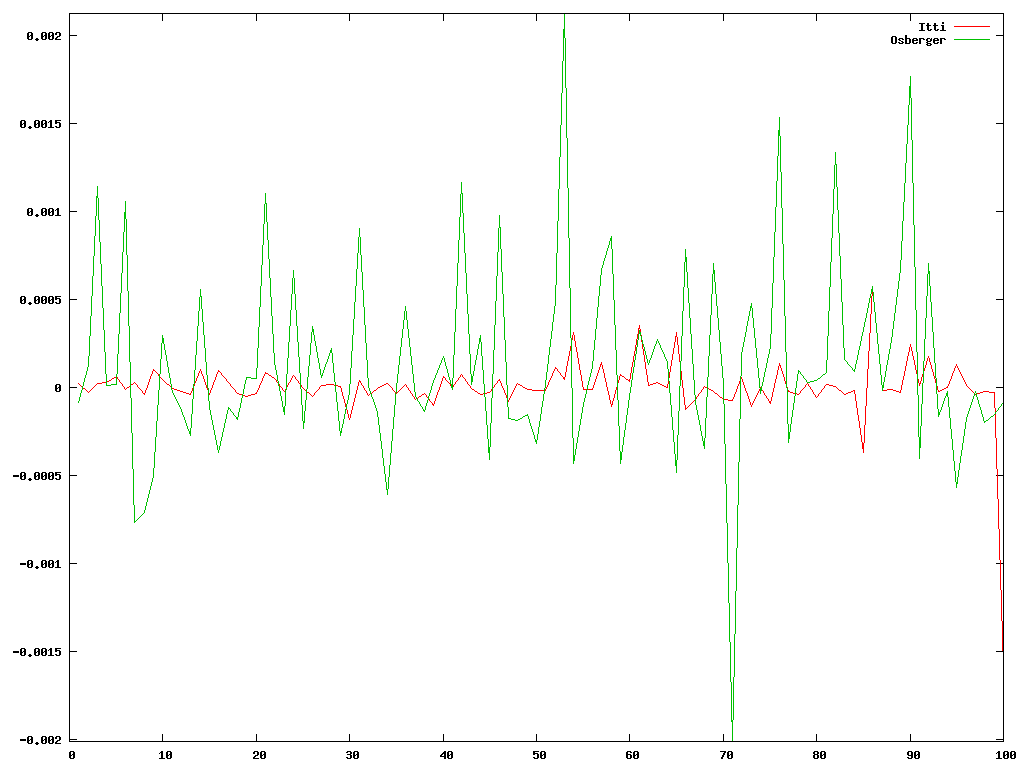
\includegraphics[width=0.45\textwidth]{images/kl}
%\caption{kl-distance}
%\label{kl}
%\end{figure}

%\begin{table}[t]
%\begin{center}
%\begin{tabular}{lcc}
%
%\hline
%                    &  {\small Itti's method}     & {\small Fuzzy growing}    \\
%\hline
%{\small Precision}           &  0.4475    & 0.4506 \\
%{\small Recall}              &  0.5515    & 0.5542 \\
%\hline
%
%\end{tabular}
%\caption[Evaluation of FOA sets]{\small Evaluation of FOA sets. } \label{t:FOA}
%\end{center}
%\end{table}

